\documentclass[../main]{subfiles}

\begin{document}

\section{Transition Metals}

	\subsection{Period 3 and the 3d Orbital}

	The 3d block contains 10 elements ranging from \ch{Sc} to \ch{Zn}, characterized by their trend to add electrons to a inner d-shell orbitals rather than to an outermost electron shell orbital.

	\subsubsection{d Orbital Shapes}

	Refer to `Orbitals' in Atomic Structure. \\

	\subsubsection{Electronic Configuration of d-block elements}

	Refer to `Electronic Configuration' in Atomic Structure. \\

	Key points to note are that \ch{Cr} and \ch{Cu} have a \usup{4s}{1} configuration. \\

	\subsubsection{The Transition Elements}

	\scidef{Transition Element}{A Transition Element is a d-block element which can form one or more stable ions with a partially filled d orbital.}

	\ch{Zn} is not a transition element as \ch{Zn2+} has a fully filled 3d orbital. \ch{Cu} may seem as if it is not a transition element as it readily forms \ch{Cu+} with a fully filled 3d orbital, but in fact it forms a stable \ch{Cu2+} with a [Ar] \usup{3d}{9} configuration and is hence a transition element. \\

	\subsection{Physical Properties of Transition Metals}

	Varying physical properties across the 3d block can be derived from numerous changing characteristics:

	\begin{description}
	\item[Number of electronically accessible electrons]:\\
		Due to the similar energy levels of the 3d and 4s electrons, both sets of electrons are available for donation and disassociation. Across the block, there is an increase in number of 3d electrons.
	\item[Number of Protons]:\\
		Number of protons increases across the block, increasing nuclear charge but also increasing the mass per atom of metal. 
	\item[Effective Nuclear Charge]:\\
		Electrons are added to the penultimate electron shell which DOES impact the amount of shielding experienced by the 4s orbital. \\
		Across the block, as nuclear charge increases and shielding effect increases, there is an overall small increase in effective nuclear charge but it is effectively constant past Group 5 elements.
	\end{description}

	\subsubsection{Melting and Boiling Points}

	Across the block, as the number of electronically accessible electrons increases, strength of metallic bonding increases, therefore requiring more thermal energy to overcome these metallic bonds and increasing both melting and boiling points across the period. \\

	\subsubsection{Electrical Conductivity}

	Across the block, as the number of electronically accessible electrons increases, the number of mobile charge carriers also increases, therefore reducing the resistance of a metal. \\

	\subsubsection{Atomic Radius}

	Atomic Radius decreases across the period as effective nuclear charge increases, but is approximately constant past Group 5.

	\subsubsection{Ionic Radius}

	Ionic Radius of the 2+ ions decreases across the 3d block. As now all 4s orbitals are vacant, ionic radius is provided by the 3d orbitals. Shielding effect only slightly increases due to 3d orbitals shielding each other but nuclear charge still increases, hence effective nuclear charge increases consistently and attraction of valence electrons increases.

	\subsubsection{Density}

	Density is determined by the atomic radius of metal atoms and their relative masses. As the atomic radius of 3d block elements is constant but their mass numbers still increase across the block, density increases across the block.

	\subsubsection{Ionization Energy}

	As effective nuclear charge slightly increases across the block, first ionization energy also gradually increases. \\

	Subsequent ionization energies of 3d block elements will be abnormally low compared to their left neighbors if they:

	\begin{itemize}
		\item Involve the ionization of a \usup{3d}{6} to \usup{3d}{5} configuration; OR
		\item Involve the ionization of a \usup{4s}{1} electron while neighbors are already removing electrons from the 3d shell (\ch{Mn} and \ch{Zn} \usup{1}{st} I.E.s).
	\end{itemize}

	\subsection{Variable Oxidation States}

	Due to the similarity of energy levels of electrons in the 3d and 4s subshells, electrons in both sets of orbitals are available for bond formation and electron donation, allowing them to display multiple oxidation states. \\

	The maximum oxidation state of the transition metals is equal to the number of unpaired d-electrons plus the two 4s electrons. \ch{Mn} is able to form the highest maximum oxidation state of +7. \\

	Compounds with TM elements in low oxidation states are typically basic (e.g. \ch{MnO}) while compounds with TM elements in high oxidation states are acidic (e.g. \ch{Mn2O6}). \\

	\subsubsection{Redox Potentials of TM Cations}

	Many of the TM elements exist in common oxidation states of +2 or +3. The relative stabilities of their +2 and +3 oxidation states can be quantified by examining their reduction potentials, where the more positive the reduction potential from +3 to +2 the more stable their +2 oxidation state. \\

	Across the d-block, the reduction potential from +3 to +2 cations becomes more positive over the group, except for \ch{Fe} which has an abnormally low reduction potential due to the transition from a \usup{3d}{5} to \usup{3d}{6} configuration being less stable due to electron repulsion within an orbital.

	\subsection{Transition Metal Catalysis}

	Transition metals are able to act as catalysts to speed up many reactions. \\

	Due to the presence of partially-filled 3d subshells, transition metals are able to exchange electrons with other molecules to form weak bonds, whether through donating 3d electrons or by accepting electrons into low-lying orbitals. These weak bonds facilitate adsorption of molecules to the surface of metals and allow for heterogeneous catalysis to occur. \\

	Common use-cases of heterogeneous catalysis include the use of powdered \ch{Ni} during reduction of alkenes and \ch{Fe}/\ch{Fe2O3} in the Haber Process. \\

	Transition metals' ability to form compounds with variable oxidation states, and the ease of reacting between these compounds mean they easily facilitate the formation and removal of intermediate compounds within a reaction as homogeneous catalysts, most commonly in reaction schemes involving redox steps. \\

	Common use-cases of homogeneous catalysis include the use of \ch{Fe3+} when encouraging the reaction of \ch{S2O8^{2-} + 2I- -> 2 SO4^{2-} + I2}. \ch{Fe3+} is an effective catalyst in this scenario as the uncatalyzed reaction has a high activation energy from the collision between two negatively charged species, while the catalyzed reaction involves two steps between anions and \ch{Fe2+}/\ch{Fe3+} cations and is hence of a much lower activation energy.

	\subsection{Transition Metal Complexes}

	\scidef{Complex}{A Complex is a chemical species which comprises of a central metal atom or ion, bonded to one or more surrounding atoms or molecules with dative covalent bonds.}

	\scidef{Complex Ion}{A Complex Ion is a Complex with a non-zero charge.}

	\scidef{Ligand}{A Ligand is a species of molecule or ion which has at least one lone pair of electrons which can be donated into a low-lying vacant orbital of a central metal atom or ion to form a dative covalent bond, thus forming a complex.}

	The number of bonds in a complex ion typically exceeds the current oxidation state of the actual metal atom. \\

	\subsubsection{Complex Formation}

	\begin{center}
		\ch{Ag^{2+} + 6 H2O <=> [Ag(H2O)6]^{2+}}
	\end{center}

	Transition Metals and their cations commonly form complexes due to the presence of low-lying vacant orbitals which can accept donated electrons from ligands,  as well as their generally large charge-to-mass ratio which can then more strongly attract electron pairs from free ligands. \\

	S-block metals typically do not form complexes as they lack the electronically accessible low-lying vacant orbitals to accept bonds from ligands, and also generally have a smaller charge-to-mass ratio which is unable to hold ligands in place.

	\subsubsection{Ligands and Complex Geometry}

	Ligands are often classified according to how many dative bonds they can form with metal atoms. Most ligands are monodentate (\ch{H2O}, \ch{OH-}, \ch{NH3}, \ch{CN-}), some are bidentate (\ch{C2O4^{2-}}), some tetradentate (haem) and some hexadentate (\ch{edta^{4-}}). \\

	\scidef{Coordination Number}{The Coordination Number of a complex is the number of dative bonds formed between the central metal atom or ion and its ligands.}

	Dative bonds of complexes (not necessarily the ligands themselves) arrange themselves around central metal ions similar to how electrons rearrange themselves into specific geometries as suggested by VESPR. Complexes with two dative bonds may have a linear geometry, four bonds may have tetrahedral or square planar geometry and six bonds may have an octahedral geometry. \\

	\subsubsection{Complex Salts}

	\scidef{Complex Salts}{Complex Salts are salts with one or more constituent complex ions.}

	Written formulas of complex salts may be ambiguous in describing how many species are ligands and how many others are anions, such as \ch{Cr(NH3)3Cl3} which is a neutral complex while \ch{Cr(NH3)5Cl3} which is a complex salt made of \ch{Cr(NH3)Cl^{2+}} and \ch{2 Cl-}. \\

	The species which is a ligand can be differentiated by species which is an ion as the ion is completely disassociated in water and can react elsewhere while the ligand is typically unreactive - in the latter case \SI{1}{\mol} of salt will form \SI{2}{\mol} of \ch{AgCl}{ppt}, with the last \ch{Cl-} being kept in the complex ion.

	\subsubsection{Common Complex Ions}

	\textbf{Bolded} ions are in the QA syllabus. \\

	\begin{tabular}{|l|l|l|}
		\hline
		Complex                           & Color      & Properties                                                        \\ \hline
		\ch{[Cu(H20)6]^{2+}}              & Light Blue & Aqua complex                                                   \\ \hline
		\textbf{\ch{[Cu(NH3)4]^{2+}}}     & Deep Blue  & Soluble in \ch{NH3}                                               \\ \hline
		\ch{[Cu(Cl)4]^{2-}}               & Yellow     & \parbox[t]{3cm}{May appear green due to mixing with aqua complex} \\ \hline
		\ch{[Cu(Cl)2]-}                   & -          & Complex of Copper (I)                                     \\ \hline
		\ch{[Ag(H2O)6]^{+}}                & Colorless  & Aqua complex                                                      \\ \hline
		\textbf{\ch{[Ag(NH3)]^{4+}}}      & Colorless  & \parbox[t]{3cm}{Complex in \ch{NH3}, used when testing halides}   \\ \hline
		\ch{[Cr(H20)6]^{3+}}              & Green      & Acidic from 3+ cation                                             \\ \hline
		\textbf{\ch{[Cr(OH)6]^{3-}}}      & Green      & Soluble in \ch{NaOH}                                              \\ \hline
		\textbf{\ch{[Cr(NH3)6]^{3+}}}     & Green      & Solbule in \ch{NH3}                                               \\ \hline
		\textbf{\ch{[Al(OH)4]^{-}}}       & Colorless  & Not a TM, but complex                                             \\ \hline
		\textbf{\ch{[Zn(OH)4]^{2-}}}      & Colorless  & Soluble in \ch{NaOH}                                              \\ \hline
		\textbf{\ch{[Zn(NH3)4]^{2+}}}     & Colorless  & Solbule in \ch{NH3}                                               \\ \hline
	\end{tabular}

	\subsection{Complex Chemistry}

	\subsubsection{Aqua Complexes}

	\scidef{Aqua Complex}{An Aqua Complex is a complex species with only \ch{H2O} as a ligand.}

	Most complexes with water have a coordination number of 6, except for \ch{Pt2+} and \ch{Pd2+}. \\

	Transition metals form aqua complexes in water, as compared to s-block metals which form hydration spheres from ion-dipole interactions. \\

	\begin{center}
		\ch{[Al(H2O)6]^{3+} + H2O -> [Al(OH)(H2O)5]^{2+} + H3O+} \\
	\end{center}

	Aqua complexes of 3+ metal cations have sufficiently large charge-to-mass ratios which give them very high polarizing power. This polarization leads to distortion of the electron clouds of \ch{H2O} ligands, wakening the \ch{O-H} bond and allowing other free \ch{H2O} molecules to take in protons from the ligands, forming \ch{H3O+}. Solutions of \ch{3+} ions are hence slightly acidic.

	\subsubsection{Ligand Exchange} 

	Ligand exchange reactions occur when one complex is formed form another, involving the removal of one species of ligand and the addition of the other. When a solution containing one complex has another ligand added to solution, further equilibriums are established involving ligand exchange.

	\begin{center}
		\ch{[Cu(H2O)]^{2+} + 4 NH3 <=> [Cu(NH3)]^{2+} + 6 H2O} \\
		\(K_{stab} = \frac{[\ch{Cu(NH3)^{2+}}]}{[\ch{Cu(H2O)6^{2+}}][\ch{NH3}]^4}\)
	\end{center}

	\scidef{Stability Constant \(K_{stab}\)}{The Stability Constant \(K_{stab}\) of the formation of a complex salt is the equilibrium constant for the formation of a new complex from an aqua complex. The greater its value, the more stable a complex is with respect to its aqua complex of the same metal ion.}

	\scieqn{Stability Constant \(K_{stab}\)}{The Stability Constant \(K_{stab}\) of the formation of a complex salt with chemical formula \ch{[M(ligand)_{\(n\)}]^{\(x\)+}}, in a solution at equilibrium with concentrations \([\ch{M(ligand)_{\(n\)}^{\(x\)+}}]\), \([\ch{M(H2O)6^{\(x\)+}}]\) and \([\ch{ligand}]\) is given by the equation}{K_{stab} = \frac{[\ch{M(ligand)^{\(x\)+}}]}{[\ch{M(H2O)6^{\(x\)+}}][\ch{ligand}]^n}}

	As with other equilibrium constants, the value of \(K_{stab}\) is constant at any given temperature and do not vary with concentration.\\

	If a solution contains ligands to form multiple possible complexes, the various \(K_{stab}\) values can be used to identify which species, generally the complex with the highest \(K_{stab}\), will be the main complex present. 

	\subsubsection{Color of Transition Metals}

	As ligands approach the central metal ion, the dative bonds formed become regions of higher electron density which then repel inner electron orbitals of the metal ion. Due to the geometry of the various 3d orbitals, electron orbitals are repelled to different extents and now have an energy gap between partially filled orbitals. Small energy gaps such as these correspond to the energies of visible light particles, allowing these central ions to now absorb energy corresponding to specific wavelengths to promote electrons from a filled to empty but higher-energy orbital, leading to the occurrence of color. \\

	Complexes with octahedral geometry have its ligands approach along the x, y and z axes, thus repelling orbitals which are along the axis more, leading to the higher energy levels of the \usup{x}{2}-\usup{y}{2} and \usup{z}{2} orbitals. Complexes with tetrahedral geometry have its ligands approach between the x, y and z axes and thus leading to higher energy levels of the xy, xz and yz orbitals.

	\begin{center} 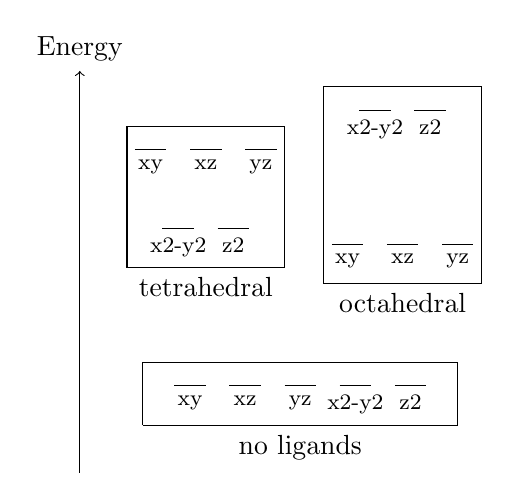
\begin{tikzpicture}

		\draw[->] (0,-0.6) -- (0,4.5) node[anchor=south] {Energy};

		\draw (0.8,0) -- (0.8,0.8) -- (4.8,0.8) -- (4.8,0) -- (0.8,0)  node [midway,anchor=north] {no ligands};

		\draw (0.6,2) -- (0.6,3.8) -- (2.6,3.8) -- (2.6,2) -- (0.6,2)  node [midway,anchor=north] {tetrahedral};

		\draw (3.1,1.8) -- (3.1,4.3) -- (5.1,4.3) -- (5.1,1.8) -- (3.1,1.8)  node [midway,anchor=north] {octahedral};

		\foreach\orbit [count=\x] in {xy, xz, yz, \usup{x}{2}-\usup{y}{2}, \usup{z}{2}} 
			\draw ({\x*0.7+0.5},0.5) -- ({\x*0.7+0.9},0.5) node[midway,anchor=north] {\footnotesize \orbit};

		\foreach\orbit [count=\x] in {xy, xz, yz} 
			\draw ({\x*0.7+0},3.5) -- ({\x*0.7+0.4},3.5) node[midway,anchor=north] {\footnotesize \orbit};

		\foreach\orbit [count=\x] in {\usup{x}{2}-\usup{y}{2}, \usup{z}{2}} 
			\draw ({\x*0.7+0.35},2.5) -- ({\x*0.7+0.75},2.5) node[midway,anchor=north] {\footnotesize \orbit};

		\foreach\orbit [count=\x] in {xy, xz, yz} 
			\draw ({\x*0.7+2.5},2.3) -- ({\x*0.7+2.9},2.3) node[midway,anchor=north] {\footnotesize \orbit};

		\foreach\orbit [count=\x] in {\usup{x}{2}-\usup{y}{2}, \usup{z}{2}} 
			\draw ({\x*0.7+2.85},4) -- ({\x*0.7+3.25},4) node[midway,anchor=north] {\footnotesize \orbit};

	\end{tikzpicture} \end{center}

	When complexes absorb color of one specific wavelength, the color that is observed later on is the complement of said absorbed color. Complementary color pairs include red-green, orange-blue and yellow-purple. \\

	Various complexes of the same central metal ion but different ligands may exhibit different colors. This is because various ligands are able to split the d orbitals to different extents. In terms of increasing splitting effect (and hence decreasing wavelength of absorbed light), the spectrochemical series orders the species of:

	\begin{center}
		Halide Anions (Starting with \ch{I}), \ch{OH-}, Ethanedioate,\\
		\ch{H2O} ,\ch{edta} ,\ch{NH3} ,\ch{NO2-} ,\ch{CN-} ,\ch{CO}
	\end{center}

	\subsubsection{Haemoglobin}

	Haemoglobin is a molecule in blood which is used in the transport of \ch{O2} around the body. Haemoglobin is a complex, with a central \ch{Fe2+} ion, one tetradentate haem ligand which surrounds the xy plane, one monodentate globin protein and finally one extra empty site for \ch{O2} ligands to bind to. The binding of \ch{O2} to haemoglobin allows for efficient transport of \ch{O2} throughout the human body via its circulatory system. \\

	Species such as \ch{CN-} and \ch{CO} are much stronger ligands than \ch{O2}, and will bind to haemoglobin molecules much more strongly than \ch{O2}. This renders the haemoglobin molecule unable to bind to and transport \ch{O2} throughout the body, leading to what we know as carbon monoxide poisoning and an additional side effect of cyanide poisoning. \\

	Other animals such as horseshoe crabs have blue-colored blood. This is due to the presence of haemocyanin, a haemoglobin-like molecule but with \ch{Cu2+} instead of \ch{Fe2+} as its central metal ion. 

\end{document}